%!TEX TS-program = xelatex
\documentclass[12pt, a4paper]{article}

%%%%%%%%%% Математика %%%%%%%%%%
\usepackage{amsmath,amsfonts,amssymb,amsthm,mathtools}

%%%%%%%%%%%%%%%%%%%%%%%% Шрифты %%%%%%%%%%%%%%%%%%%%%%%%%%%%%%%%%
\usepackage[british,russian]{babel} % выбор языка для документа
\usepackage[utf8]{inputenc} % задание utf8 кодировки исходного tex файла
\usepackage[X2,T2A]{fontenc}        % кодировка

\usepackage{fontspec}         % пакет для подгрузки шрифтов
\setmainfont{Arial}   % задаёт основной шрифт документа

\usepackage{unicode-math}     % пакет для установки математического шрифта
\setmathfont{Asana Math}      % шрифт для математики
% \setmathfont[math-style=ISO]{Asana Math}
% Можно делать смену начертания с помощью разных стилей


\usepackage[paper=a4paper,top=13.5mm, bottom=13.5mm, left=16.5mm, right=13.5mm, includefoot]{geometry}
\usepackage[unicode,colorlinks=true,urlcolor=blue,hyperindex,breaklinks]{hyperref}

\usepackage{indentfirst} % установка отступа в первом абзаце главы!!!
\usepackage{booktabs} 
\usepackage{float}


\title{Отчёт о проделанной работе}
\author{Винни-Пух}
\date{\today}
\begin{document}

\maketitle

\section{Основовы}




\section{Первый чанк или четыре лапки равно собачка}

Тут можно писать текст, и даже вот такие вот формулы

\[ \int_{0}^{+\infty} x^{s-1} \cdot e^{-x} dx = \Gamma(s). \]

Всё совсем как в \LaTeX! Но у нас нет на это времени! Пора создавать чанк!


\begin{knitrout}
\definecolor{shadecolor}{rgb}{0.969, 0.969, 0.969}\color{fgcolor}\begin{kframe}
\begin{alltt}
\hlstd{x} \hlkwb{<-} \hlkwd{rnorm}\hlstd{(}\hlnum{100}\hlstd{)}
\hlstd{x_mean} \hlkwb{<-} \hlkwd{mean}\hlstd{(x)}
\hlstd{x_mean}
\end{alltt}
\begin{verbatim}
## [1] 0.07131877
\end{verbatim}
\end{kframe}
\end{knitrout}

Мы видим, что наши вычисления прошли усспешно и среднее составило 0.0713188



\section{Картинки, таблицы и другие штуки!}

\begin{knitrout}
\definecolor{shadecolor}{rgb}{0.969, 0.969, 0.969}\color{fgcolor}\begin{kframe}


{\ttfamily\noindent\bfseries\color{errorcolor}{\#\# Error in curl::curl\_download(cu, tmp, handle = h): Could not resolve host: finance.yahoo.com}}

{\ttfamily\noindent\bfseries\color{errorcolor}{\#\# Error in time(GOOG): объект 'GOOG' не найден}}

{\ttfamily\noindent\bfseries\color{errorcolor}{\#\# Error in df[, -c(6, 7)]: объект типа 'closure' не делится на подгруппы}}\end{kframe}
\end{knitrout}


\begin{table}[h!]
\begin{center}

\begin{tabular}{l}
\hline
\\
\hline
function (x, df1, df2, ncp, log = FALSE)\\
\hline
\{\\
\hline
if (missing(ncp))\\
\hline
.Call(C\_df, x, df1, df2, log)\\
\hline
else .Call(C\_dnf, x, df1, df2, ncp, log)\\
\hline
\}\\
\hline
\end{tabular}


\caption{Стоимость акций}
\end{center} 
\end{table}


Таблицы можно получать немного иначе. С помощью пакета xtable. Посмотрим как! Оценим модель с помощью следующего кода: 

\begin{knitrout}
\definecolor{shadecolor}{rgb}{0.969, 0.969, 0.969}\color{fgcolor}\begin{kframe}
\begin{alltt}
\hlstd{formula} \hlkwb{=} \hlstr{"GOOG.Open~t+GOOG.Close"}
\hlstd{model} \hlkwb{<-} \hlkwd{lm}\hlstd{(}\hlkwc{data}\hlstd{=df,formula)}
\end{alltt}


{\ttfamily\noindent\bfseries\color{errorcolor}{\#\# Error in terms.formula(formula, data = data): аргумент 'data' неправильного типа}}\end{kframe}
\end{knitrout}


Оценки, которые мы заслужили приведены в таблице \ref{tab:regress}. 

\begin{kframe}


{\ttfamily\noindent\bfseries\color{errorcolor}{\#\# Error in summary(model): объект 'model' не найден}}\end{kframe}


\begin{kframe}


{\ttfamily\noindent\bfseries\color{errorcolor}{\#\# Error in summary(model): объект 'model' не найден}}\end{kframe}

Графики можно построить совсем разными. Например, вот такой! 


\begin{knitrout}
\definecolor{shadecolor}{rgb}{0.969, 0.969, 0.969}\color{fgcolor}\begin{kframe}


{\ttfamily\noindent\bfseries\color{errorcolor}{\#\# Error in if (is.waive(data) || empty(data)) return(cbind(data, PANEL = integer(0))): пропущенное значение, а нужно TRUE/FALSE}}\end{kframe}

{\centering 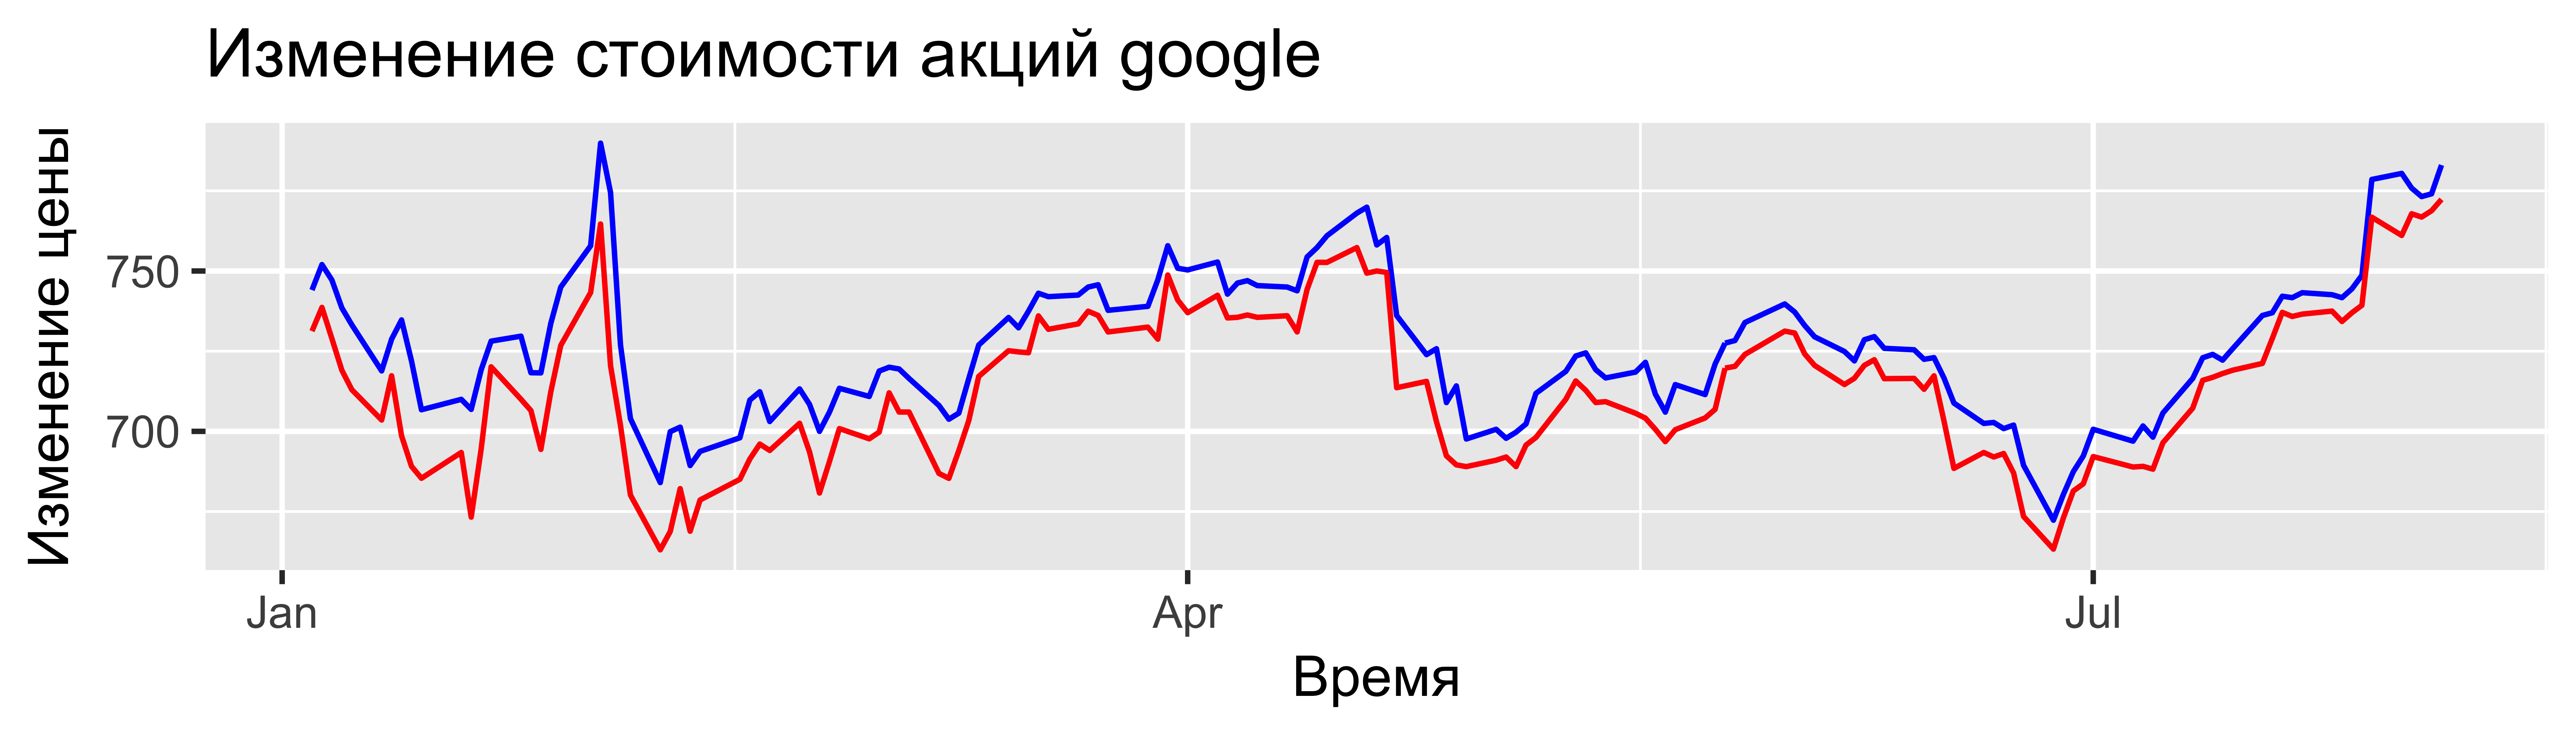
\includegraphics[width=\maxwidth]{figure/unnamed-chunk-7-1} 

}



\end{knitrout}

Можно к коду использовать любые окружения теха! Прямо как к рисунку \ref{fig}.

\begin{figure}[h!]
\begin{knitrout}
\definecolor{shadecolor}{rgb}{0.969, 0.969, 0.969}\color{fgcolor}\begin{kframe}


{\ttfamily\noindent\bfseries\color{errorcolor}{\#\# Error in eval(aesthetics\$x, data, env): неправильный аргумент 'envir' типа 'closure'}}\end{kframe}
\end{knitrout}



